\section{Applications of Differentiation}

\subsection{Position, Velocity and Acceleration}
\begin{itemize}
	\item \textbf{Position} is where something is at a specific time. It is represented by a function $x(t)$, where $t$ is time.

	\item \textbf{Velocity} is the rate of change of an object's position, or the derivative of position: $v(t) = x'(t)$. It represents how fast something is moving at a specific time. Depending on the sign of velocity, the object can be moving in different directions:
	\[ v(t) \begin{cases}
		< 0 \; \Rightarrow \; \text{moving left} \\
		= 0 \; \Rightarrow \; \text{not moving} \\
		> 0 \; \Rightarrow \; \text{moving right}
	\end{cases} \]

	\item \textbf{Acceleration} is the rate of change of an object's velocity, or the derivative of velocity: $a(t) = v'(t) = p''(t)$. It represents how fast something is changing speed at a specific time. If the sign of acceleration is the same as velocity, the object is speeding up. If the two signs are different, the object is slowing down. Finally, if the acceleration is $0$, it means that the object is moving at a constant velocity. This is visualized in Figure \ref{fig:acceleration}.
	\begin{figure}[H]
		\begin{center}
			\frame{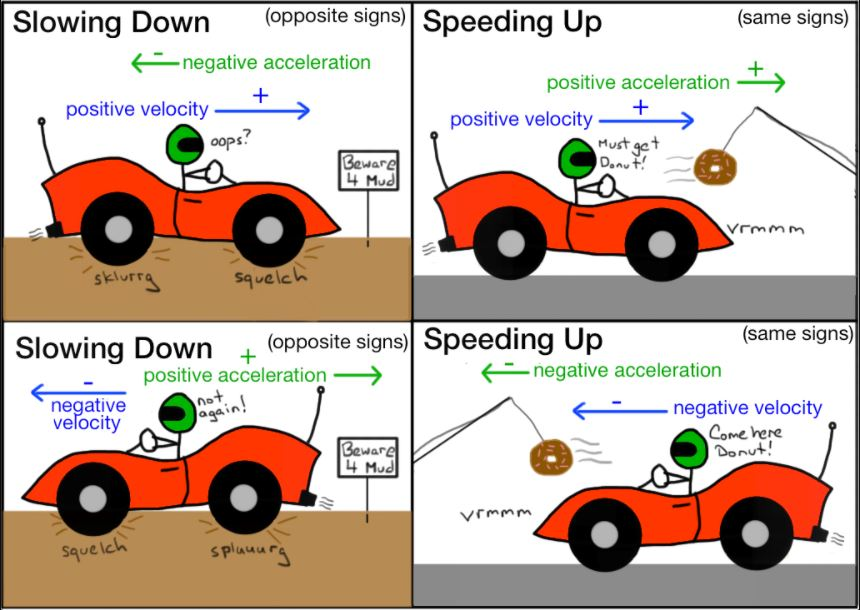
\includegraphics[width=0.6\textwidth]{images/fig4.JPG}}
			\caption{An explanation of acceleration.}
			\label{fig:acceleration}
		\end{center}
	\end{figure}
\end{itemize}

\subsection{Related Rates}
Related rates involve problems which involve two quantities that are changing at the same time. Given that the two rates are related, we can figure out how fast one of them is changing based on how fast the other is changing. This is usually done by implicitly differentiating a relation equation with respect to time, $t$.

\noindent \textbf{Examples:}
\begin{enumerate}
	\item Given the equation: $\frac{x}{y} = 9$, and $\frac{dy}{dt} = -\frac{2}{3}$, find $\frac{dx}{dt}$ when $x = 3$.

	To begin, implicitly differentiate the given equation $\frac{x}{y} = 9$ with respect to $t$:
	\begin{align*}
		\frac{x}{y} &= 9 \\[5pt]
		\frac{y \cdot \frac{dx}{dt} - x \cdot \frac{dy}{dt}}{y^2} &= 0 \\[5pt]
		y \cdot \frac{dx}{dt} - x \cdot \frac{dy}{dt} &= 0.
	\end{align*}

	In this new equation, there are two unknowns: $\frac{dx}{dt}$ and $y$. To solve for $\frac{dx}{dt}$, we first have to solve for $y$:
	\begin{align*}
		\frac{x}{y} &= 9 \\[5pt]
		y &= \frac{x}{9} \\[5pt]
		y &= \frac{3}{9} \\[5pt]
		y &= \frac{1}{3}
	\end{align*}

	Finally, solving for $\frac{dx}{dt}$:
	\begin{align*}
		y \cdot \frac{dx}{dt} - x \cdot \frac{dy}{dt} &= 0 \\[5pt]
		\frac{dx}{dt} &= \frac{x \cdot \frac{dy}{dt}}{y} \\[5pt]
		\frac{dx}{dt} &= \frac{3 \cdot \left( -\frac{2}{3} \right)}{\frac{1}{3}} \\[5pt]
		\frac{dx}{dt} &= -6
	\end{align*}

	\item The surface area of a sphere is increasing at a rate of $14 \pi$ square meters per hour. At a certain instant, the surface area is $36 \pi$ square meters. What is the rate of change of the volume of the sphere at that instant?

	First, list out relevant equations, and implicitly differentiate them with respect to time:
	\begin{itemize}
		\item Surface area, $SA$, of a sphere with radius $r$:
		\begin{align*}
			SA &= 4 \pi r^2 \\
			\frac{dSA}{dt} &= 8 \pi r \cdot \frac{dr}{dt}.
		\end{align*}

		\item Volume, $V$, of a sphere with radius $r$:
		\begin{align*}
			V &= \frac{4}{3} \pi r^3 \\[5pt]
			\frac{dV}{dt} &= 4 \pi r^2 \cdot \frac{dr}{dt}.
		\end{align*}
	\end{itemize}

	Within these four equations, there are several unknowns:
	\begin{itemize}
		\item The radius of the sphere, $r$.
		\item The rate of change of radius, $\frac{dr}{dt}$.
		\item The rate of change of volume, $\frac{dV}{dt}$.
	\end{itemize}

	Solving for $r$:
	\begin{align*}
		SA &= 4 \pi r^2 \\
		r^2 &= \frac{SA}{4 \pi} \\[5pt]
		r &= \sqrt{\frac{SA}{4 \pi}} \\[5pt]
		r &= \sqrt{\frac{36 \pi}{4 \pi}} \\[5pt]
		r &= 3
	\end{align*}

	Solving for $\frac{dr}{dt}$:
	\begin{align*}
		\frac{dSA}{dt} &= 8 \pi r \cdot \frac{dr}{dt} \\[5pt]
		\frac{dr}{dt} &= \frac{\frac{dSA}{dt}}{8 \pi r} \\[5pt]
		\frac{dr}{dt} &= \frac{14 \pi}{8 \pi \cdot 3} \\[5pt]
		\frac{dr}{dt} &= \frac{7}{12}
	\end{align*}

	Finally, solving for $\frac{dV}{dt}$:
	\begin{align*}
		\frac{dV}{dt} &= 4 \pi r^2 \cdot \frac{dr}{dt} \\[5pt]
		\frac{dV}{dt} &= 4 \pi \cdot 3^2 \cdot \frac{7}{12} \\[5pt]
		\frac{dV}{dt} &= 21 \pi
	\end{align*}

	Therefore, at this instance in time, the volume of the sphere is changing by $21 \pi$ meters cubed.
\end{enumerate}

\subsection{Local Linearity and Approximation}
Local linearity is the graphical representation of a derivative. By zooming in really close to a function that is differentiable on all points in its domain, it would eventually become a straight line. It is much easier to work with this straight line as a slope for approximating other values.

Given a function $f(x)$, the equation of the tangent line at a point where $x = a$ is given below. Notice that this equation resembles the point-slope form equation, $y = m(x - x_1) - y_1$. The slope, $m$, is the derivative at point $a$, $f'(a)$.
\[ y = f'(a) (x - a) + f(a) \]

This can be useful in approximating values on a graph that are close another, known value. For example, in Figure \ref{fig:linearity}, there is a graph with function $f(x) = \sqrt{x}$. The value of point $A$ is $\sqrt{0.25} = 0.5$. However, the point $B$ is at $\sqrt{0.3}$, which is harder to calculate. However, it can be observed that the tangent line at point $A$ comes really close to point $B$, so we can use local linearity to approximate the value of $B$.

\begin{figure}[H]
	\begin{center}
		\frame{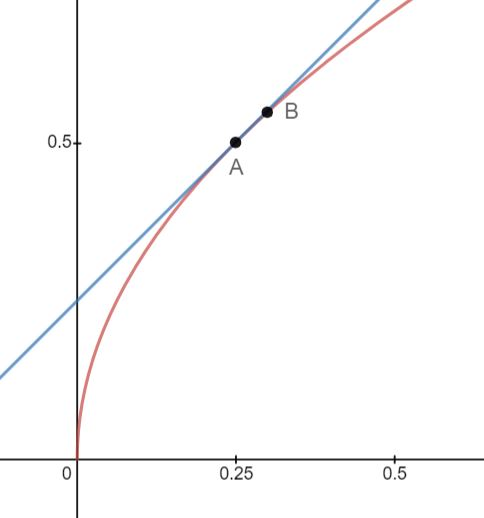
\includegraphics[width=0.4\textwidth]{images/fig5.JPG}}
		\caption{A demonstration of local linearity.}
		\label{fig:linearity}
	\end{center}
\end{figure}

The first step is to find the value of the slope at point $A$. This can be done by finding the value of the derivative at $x_A = 0.25$, or $f'(0.25)$.
\begin{align*}
	f(x) &= \sqrt{x} \\
	f'(x) &= \frac{1}{2} \cdot x^{-\frac{1}{2}} \\[5pt]
	f'(x) &= \frac{1}{2 \sqrt{x}} \\[5pt]
	f'(0.25) &= 1
\end{align*}

With this, we can plug in all required values into the local linearity line equation to get the equation of the tangent at point $A$.
\begin{align*}
	y &= f'(0.25) (x - 0.25) + f(0.25) \\
	y &= 1 (x - 0.25) + \sqrt{0.25} \\
	y &= x + 0.25
\end{align*}

Finally, to find the $y$ value of point $B$, substitute in the $x$ value of point $B$ into the above equation.
\begin{align*}
	y_B &= x_B + 0.25 \\
	y_B &= 0.3 + 0.25 \\
	y_B &= 0.55
\end{align*}

Therefore, point $B$ is located at approximately $(0.3, 0.55)$. Using a calculator reveals that the actual value of $B$ is $(0.3, 0.547)$, which is really close to the approximation.

\subsection{L'Hopital's Rule}
L'Hopital's rule allows the evaluation of limits in indeterminate forms. It states the following:
\begin{gather*}
	\text{if} \\
	\lim_{x \to c} \frac{f(x)}{g(x)} = \frac{0}{0} \quad \text{or} \quad \lim_{x \to c} \frac{f(x)}{g(x)} = \frac{\pm \infty}{\pm \infty} \\
	\text{then} \\
	\lim_{x \to c} \frac{f(x)}{g(x)} = \lim_{x \to c} \frac{f'(x)}{g'(x)}.
\end{gather*}

Note that l'Hopital's rule only applies if direct substitution of the limit evaluates to an indeterminate form. That is, if direct substitution gives a definite value, l'Hopital's rule will not work.

\noindent \textbf{Examples:}

\begin{enumerate}
	\item Find the value of $\lim \limits_{x \to 0} \frac{\sin x}{x}$.

	Direct substitution results in indeterminate form:
	\[ \lim_{x \to 0} \frac{\sin x}{x} = \frac{\sin 0}{0} = \frac{0}{0}. \]

	Using l'Hopital's rule, take the derivative of the numerator and denominator, separately. Then, reevaluate the limit:
	\begin{align*}
		\lim_{x \to 0} \frac{\sin x}{x} &= \lim_{x \to 0} \frac{\cos x}{1} \\[5pt]
		&= \frac{\cos 0}{1} \\[5pt]
		\lim_{x \to 0} \frac{\sin x}{x} &= 1.
	\end{align*}

	\item Find the value of $\lim \limits_{x \to \infty} \frac{e^x}{x^2}$.

	Direct substitution results in indeterminate form:
	\[ \lim_{x \to \infty} \frac{e^x}{x^2} = \frac{e^\infty}{\infty^2} = \frac{\infty}{\infty}. \]

	As with before, use l'Hopital's rule to take the derivative of the numerator and denominator. Then, reevaluate the limit:
	\[ \lim_{x \to \infty} \frac{e^x}{x^2} = \lim_{x \to \infty} \frac{e^x}{2x}. \]

	However, this limit still results in indeterminate form:
	\[ \lim_{x \to \infty} \frac{e^x}{2x} = \frac{e^\infty}{2 \cdot \infty} = \frac{\infty}{\infty}. \]

	Simply apply l'Hopital's rule again, then reevaluate the limit:
	\begin{align*}
		\lim_{x \to \infty} \frac{e^x}{2x} &= \lim_{x \to \infty} \frac{e^x}{2} \\[5pt]
		&= \frac{\infty}{2} \\[5pt]
		\lim_{x \to \infty} \frac{e^x}{2x} &= \infty.
	\end{align*}

	Therefore, the value of the original limit is also $\infty$.
\end{enumerate}

\subsubsection{Other Indeterminate Forms}
L'Hopital's rule can also be used to find limits involving exponential functions $f(x)^{g(x)}$. When taking the limit, the functions approach one of the following sets of values:

\begin{enumerate}
	\item $f(x) \to 0$ and $g(x) \to 0$
	\item $f(x) \to 1$ and $g(x) \to \infty$
	\item $f(x) \to \infty$ and $g(x) \to 0$
\end{enumerate}

Let $y = f(x)^{g(x)}$, and take the natural log of both sides. Rearrange and use l'Hopital's rule to solve the limit.
\begin{align*}
	y &= f(x)^{g(x)} \\
	\ln y &= g(x) \ln f(x) \\
	\lim_{x \to c} \ln y &= \lim_{x \to c} g(x) \ln f(x)
\end{align*}

\noindent For example, find the limit $\lim \limits_{x \to 0^+} x^x$.
\begin{align*}
	y &= x^x \\
	\ln y &= x \ln x \\
	\lim_{x \to 0^+} \ln y &= \lim_{x \to 0^+} x \ln x
\end{align*}

\noindent An attempt at direct substitution on the right-hand side results in an unfamiliar indeterminate form, $0 \times (- \infty)$. To solve this, rearrange the right-hand side to involve a fraction.
\[ \lim_{x \to 0^+} \ln y = \lim_{x \to 0^+} \frac{\ln x}{\frac{1}{x}}. \]

\noindent Now, direct substitution results in a workable indeterminate form:
\[ \lim_{x \to 0^+} \frac{\ln x}{\frac{1}{x}} = -\frac{\infty}{\infty}. \]

\noindent We can apply l'Hopital's rule again to solve this limit:
\begin{align*}
	\lim_{x \to 0^+} \ln y &= \lim_{x \to 0^+} \frac{\ln x}{\frac{1}{x}} \\[5pt]
	&= \lim_{x \to 0^+} \frac{\frac{1}{x}}{-\frac{1}{x^2}} \\[5pt]
	&= \lim_{x \to 0^+} -x \\
	\lim_{x \to 0^+} \ln y &= 0
\end{align*}

\noindent Finally, substitute this back into the original equation to find the limit $\lim \limits_{x \to 0^+} x^x$:
\begin{align*}
	\lim_{x \to 0^+} x^x &= \lim_{x \to 0^+} y \\
	&= \lim_{x \to 0^+} e^{\ln y} \\
	&= e^{\left( \lim \limits_{x \to 0^+} \ln y \right)} \\
	&= e^0 \\
	\lim_{x \to 0^+} x^x &= 1
\end{align*}

\noindent Note that in the step involving moving the limit operator inside the exponent:
\[ \lim_{x \to 0^+} e^{\ln y} = e^{\left( \lim \limits_{x \to 0^+} \ln y \right)}, \]
this is justified by the continuity of the function $e^x$. That is, $e^x$ is continuous everywhere including at $\lim \limits_{x \to 0^+} \ln y$, allowing the movement of the limit.

\subsection{Mean Value Theorem}
The mean value theorem states that for any arc between two endpoints on a graph, there will be a point whose tangent line is parallel to the secant line between the two endpoints.

\begin{figure}[H]
	\centering
	\frame{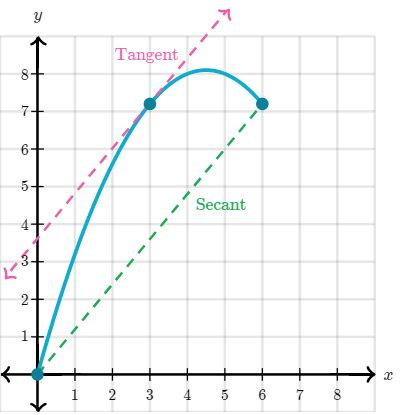
\includegraphics[width=0.4\textwidth]{images/fig6.JPG}}
	\caption{The mean value theorem.}
	\label{fig:mean_value_theorem}
\end{figure}

More precisely, given a \textit{continuous and differentiable} function $f(x)$ in the interval $[a, b]$, there exists a value $x = c, \; c \in [a, b]$ such that $f'(c)$ is equal to the average rate of change over $[a, b]$.
\[ f'(c) = \frac{f(b) - f(a)}{b - a}. \]

\subsection{Extreme Value Theorem}
If $f(x)$ is a continuous function over the closed interval $[a, b]$, then there exists a maximum and minimum value of $f(x)$. More formally, there much exist numbers $c$ and $d$ in $[a, b]$ such that $f(c) \leq f(x) \leq f(d)$ for all $x \in [a, b]$.

\subsection{First Derivative, Second Derivative and Candidates Tests}
The first derivative test, second derivative test, and candidates test are used together to find relative (or local) and absolute (or global) extrema in a function.

\subsubsection{Relative and Local Extrema}
A \textit{relative} maximum is a point on a graph where the function is the largest, relative to its immediate left and right. At this point, the function changes from increasing to decreasing. Similarly, a relative minimum is a point on a graph where the value of the function is the smallest, relative to its immediate left and right. At this point, the function changes from decreasing to increasing.

Points of extrema, such as a maximum or minimum, alongside points of inflection, are all categorized as critical points. Such points occur when the first derivative of the function is $0$ or undefined. Therefore, we can use the \textbf{first derivative test} to find extrema. For example, find the relative extremum of $f(x) = \frac{x^2}{x - 1}$.
\begin{align*}
	f(x) &= \frac{x^2}{x - 1} \\[5pt]
	f'(x) &= \frac{x^2 - 2x}{(x - 1)^2}
\end{align*}

\noindent The critical points occur at when $f'(x)$ is $0$ or undefined.
\begin{table}[H]
	\centering
	\begin{tabular}{|c|c|}
		\hline
		$x$ & $f'(x)$ \\
		\hline \hline
		$0, 2$ & $0$ \\
		\hline
		$1$ & undefined \\
		\hline
	\end{tabular}
\end{table}

\noindent Next, test the intervals between the critical points to see whether they are at a maximum, minimum, or point of inflection. This can be done by testing to see if the function is increasing ($f'(x) > 0$), or decreasing ($f'(x) < 0$) at each interval. Simply pick a random number in the interval and see if it is positive or negative.
\begin{table}[H]
	\centering
	\begin{tabular}{|c|c|c|}
		\hline
		Interval & $f'(x)$ & Slope of $f(x)$ \\
		\hline \hline
		$(-\infty, 0)$ & $+$ & $\nearrow$ \\
		\hline
		$(0, 1)$ & $-$ & $\searrow$ \\
		\hline
		$(1, 2)$ & $-$ & $\searrow$ \\
		\hline
		$(2, \infty)$ & $+$ & $\nearrow$ \\
		\hline
	\end{tabular}
\end{table}

\noindent At $x = 0$, $f'(x)$ switches from positive to negative, so $f(x)$ has a relative maximum. Similarly, at $x = 2$, $f'(x)$ switches from negative to positive, so $f(x)$ has a relative minimum. The sign of $f'(x)$ does not change at $x = 1$, so $f(x)$ experiences neither a relative maximum nor minimum, but rather a point of inflection (discussed in \ref{sec:concavity}).

An alternative, easier method for determining the nature of a critical point is the \textbf{second derivative test}. The second derivative is the change in the first derivative. Therefore, the sign of the second derivative determines whether the slope of the function is increasing or decreasing (not positive or negative). Given a point where $f'(x) = 0$, then:
\[ f''(x) \begin{cases}
	> 0 \Rightarrow \text{minimum point at } x \\
	< 0 \Rightarrow \text{maximum point at } x \\
	= 0 \Rightarrow \text{test is inconclusive}
\end{cases} \]

\subsubsection{Absolute and Global Extrema}
An \textit{absolute} extremum is a point where the function is at its largest or smallest across its entire domain. The method for finding absolute extrema is similar to that for finding relative ones, but with the extra consideration for the endpoints of the domain. For example, find the absolute extrema of $f(x) = x^3 + 2x^2$ for $-2 \leq x \leq 1$:

\noindent To begin, we can use the first derivative test to find the critical points:
\begin{align*}
	f(x) &= x^3 + 2x^2 \\
	f'(x) &= 3x^2 + 4x.
\end{align*}

\noindent Find the values for which $f'(x)$ is $0$ or undefined, the critical points:
\begin{table}[H]
	\centering
	\begin{tabular}{|c|c|}
		\hline
		$x$ & $f'(x)$ \\
		\hline \hline
		$-\frac{4}{3}, 0$ & $0$ \\
		\hline
	\end{tabular}
\end{table}

\noindent Determine the nature of the critical points using the second derivative test:
\begin{align*}
	f'(x) &= 3x^2 + 4x \\
	f''(x) &= 6x + 4
\end{align*}
\begin{table}[H]
	\centering
	\begin{tabular}{|c|c|}
		\hline
		$x$ & $f''(x)$ \\
		\hline \hline
		$-\frac{4}{3}$ & $-$ \\
		\hline
		$0$ & $+$ \\
		\hline
	\end{tabular}
\end{table}

\noindent This test concludes that $f(x)$ has a \textit{relative} maximum at $x = -\frac{4}{3}$ and a \textit{relative} minimum at $x = 0$. In order to find the global extrema, we have to consider the $y$ values of these points alongside $x = -2$ and $x = 1$, the endpoints of the closed interval.
\begin{table}[H]
	\centering
	\begin{tabular}{|c|c|}
		\hline
		$x$ & $y = f(x)$ \\
		\hline \hline
		$-2$ & $0$ \\
		\hline
		$-\frac{4}{3}$ & $\frac{32}{27} \approx 1.19$ \\
		\hline
		$0$ & $0$ \\
		\hline
		$1$ & $3$ \\
		\hline
	\end{tabular}
\end{table}

\noindent Therefore, it can be concluded that the absolute maximum of $f(x)$ is at $x = 1$. The $y$ values for $x = -2$ and $x = 0$ are the same, so both are absolute minimums. The function $f(x)$ is shown in Figure \ref{fig:global_extrema}.
\begin{figure}[H]
	\centering
	\frame{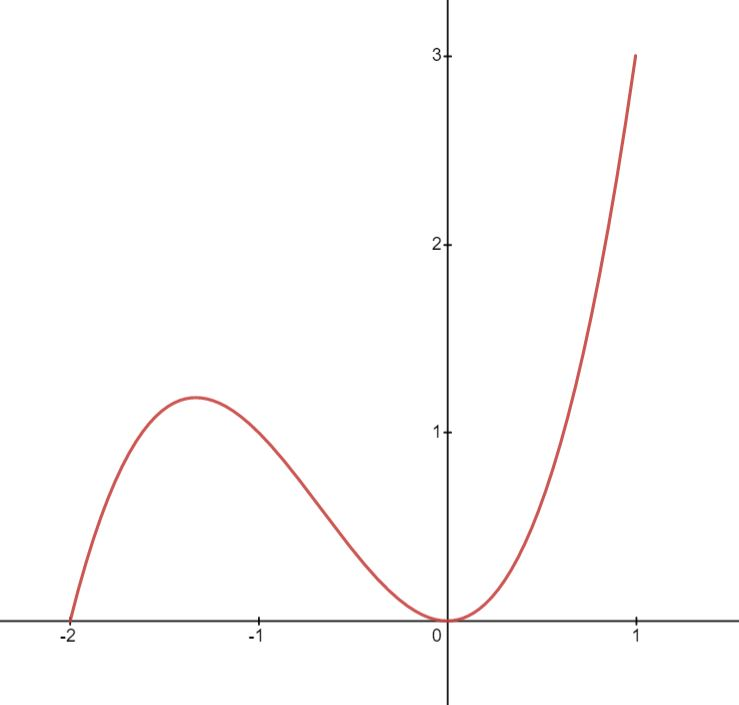
\includegraphics[width=0.4\textwidth]{images/fig7.JPG}}
	\caption{$f(x) = x^3 + 2x^2 \{ -2 \leq x \leq 1 \}$}
	\label{fig:global_extrema}
\end{figure}

\subsubsection{Concavity and Points of Inflection}
\label{sec:concavity}
Concavity is the sign of curvature of a function. Parts of a graph can either be \textit{concave up} or \textit{concave down}. When the concavity is concave up, the first derivative is increasing, thus the second derivative is positive. Inversely, when the concavity is concave down, the first derivative is decreasing, thus the second derivative is negative.

Inflection points are where the concavity flips. That is, at a point of inflection, the second derivative equals $0$. Furthermore, the sign of the second derivative changes.

\begin{figure}[H]
	\begin{center}
		\frame{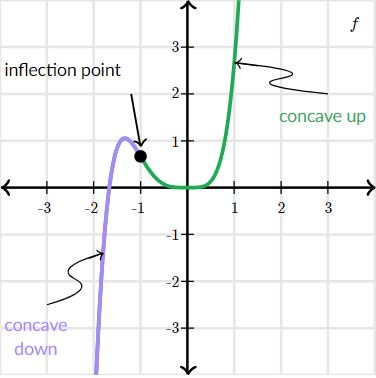
\includegraphics[width=0.4\textwidth]{fig8.JPG}}
		\caption{Concavity and points of inflection.}
		\label{fig:concavityinflection}
	\end{center}
\end{figure}

\subsection{Optimization Problems}
Optimization problems involve finding the largest or smallest something can be. This can be done by first find a function $f(x)$ to model the relationship between variables, then using $f'(x)$ to find the extrema.

\noindent \textbf{Examples:}
\begin{enumerate}
	\item Find the value of $x$ for which $y = 2x + 3$ is the closest to the origin.

	First, we can model the distance from a point $(x, y)$ to the origin, $(0, 0)$. This is given by:
	\[ D = \sqrt{x^2 + y^2}. \]

	Substitute in the given equation to get $D$ in terms of just $x$:
	\begin{align*}
		D &= \sqrt{x^2 + y^2} \\
		&= \sqrt{x^2 + (2x + 3)^2} \\
		D &= \sqrt{5x^2 + 12x + 9}.
	\end{align*}

	In order to find the minimum value of $D$, we can solve for the value of $x$ for which $\frac{dD}{dx} = 0$. First taking the derivative of $D$ with respect to $x$:
	\begin{align*}
		D &= \sqrt{5x^2 + 12x + 9} \\
		\frac{dD}{dx} &= \frac{5x + 6}{\sqrt{5x^2 + 12x + 9}}.
	\end{align*}

	Next finding the point where the derivative is $0$:
	\begin{align*}
		\frac{dD}{dx} &= 0 \\[5pt]
		\frac{5x + 6}{\sqrt{5x^2 + 12x + 9}} &= 0 \\[5pt]
		5x + 6 &= 0 \\
		x &= -\frac{6}{5}.
	\end{align*}

	We can use the second derivative test to determine whether $x = -\frac{6}{5}$ is a minimum value:
	\begin{align*}
		\frac{dD}{dx} &= \frac{5x + 6}{\sqrt{5x^2 + 12x + 9}} \\[5pt]
		\frac{d^2 D}{dx^2} &= \frac{9}{\left( 5x^2 + 12x + 9 \right)^{\frac{3}{2}}} \\[5pt]
		\frac{d^2 D}{dx^2} \Big|_{x = -\frac{6}{5}} &\approx 3.7.
	\end{align*}

	The second derivative is greater than $0$ at $x = -\frac{6}{5}$, so it can be concluded that this point is indeed a minimum point. Therefore, the function $y = 2x + 3$ will be closest to the origin at $x = -\frac{6}{5}$.

	\item Find the maximum product of two positive numbers whose sum if $300$.

	This question asks for a maximum $a \cdot b$ given $a + b = 300$. The first step if to represent the product in terms of a function of just one variable, $f(a)$.
	\begin{align*}
		b &= 300 - a \\
		ab &= a (300 - a) \\
		f(a) &= a (300 - a) \\
		f(a) &= 300a - a^2
	\end{align*}

	We can follow the same stems as the previous example to find the maximum of $f(a)$. First find the derivative of $f(a)$:
	\begin{align*}
		f(a) &= 300a - a^2 \\
		f'(a) &= 300 - 2a.
	\end{align*}

	Next, find the critical points:
	\begin{align*}
		f'(a) &= 0 \; \text{(or undefined)} \\
		300 - 2a &= 0 \\
		a &= 150.
	\end{align*}

	Use the second derivative test to validate that $a = 150$ is a maximum point:
	\begin{gather*}
		f'(a) = 300 - 2a \\
		f''(a) = -2 \\
		f''(a) < 0 \spacedforall x \in \R.
	\end{gather*}

	Therefore, the value of $a$ that yields a maximum product is $150$. Now to find $b$:
	\begin{align*}
		a + b &= 300 \\
		150 + b &= 300 \\
		b &= 150.
	\end{align*}

	Finally, the two positive integers whose sum if $300$ and yield a maximum product are $150$ and $150$.

	\item We want to construct a cylindrical can with a bottom but no top that will have a volume of $30 \mathrm{cm^3}$. Determine the dimensions of the can that will minimize the amount of material needed to construct the can.

	First, we can list out the equations for the volume ($V$), and surface area ($SA$) of the specified can:
	\begin{gather*}
		V = \pi r^2 h \\
		SA = \pi r^2 + 2 \pi r h.
	\end{gather*}

	What we are trying to minimize in this question is the surface area. To begin, we can rewrite the $SA$ equation in terms of just one variable, $r$. First we can solve for $h$ in terms of $r$:
	\begin{align*}
		\pi r^2 h &= V \\
		\pi r^2 h &= 30 \\
		h &= \frac{30}{\pi r^2}.
	\end{align*}

	Next, rewrite the equation for $SA$ as a function of $r$:
	\begin{align*}
		SA &= \pi r^2 + 2 \pi r h \\
		SA(r) &= \pi r^2 + 2 \pi r \cdot \frac{30}{\pi r^2} \\[5pt]
		SA(r) &= \pi r^2 + \frac{60}{r}.
	\end{align*}

	Take the derivative of $SA(r)$:
	\begin{align*}
		SA(r) &= \pi r^2 + \frac{60}{r} \\[5pt]
		SA'(r) &= 2 \pi r - \frac{60}{r^2}.
	\end{align*}

	Find critical points:
	\begin{align*}
		SA'(r) &= 0 \\
		2 \pi r - \frac{60}{r^2} &= 0 \\
		2 \pi r^3 - 60 &= 0 \\
		r^3 &= \frac{30}{\pi} \\
		r &= \sqrt[3]{\frac{30}{\pi}}.
	\end{align*}

	Furthermore, $SA'(r)$ would be undefined at $r = 0$. However, the radius of a cylinder can not be $0$, so this would not actually be a valid critical point. We can use the second derivative test to validate the critical point $r = \sqrt[3]{\frac{30}{\pi}}$:
	\begin{gather*}
		SA''(r) = 2 \pi + \frac{120}{r^3} \\[5pt]
		SA'' \left( \sqrt[3]{\frac{30}{\pi}} \right) > 0
	\end{gather*}

	Therefore, $r = \sqrt[3]{\frac{30}{\pi}}$ would yield the least material used for the cylinder. Going back to solve for $h$:
	\begin{align*}
		h &= \frac{30}{\pi r^2} \\
		h &\approx 2.12.
	\end{align*}
\end{enumerate}

\subsection{Behaviors of Implicit Relations}
Implicit relations are equations that can not the rewritten to have one variable in terms of the other. They can be useful in solving for unknown values or line equations. When working with implicit relations and their derivatives, the key takeaway is that variables in the original equation and higher derivatives can be substituted both ways.

\noindent \textbf{Examples:}
\begin{enumerate}
	\item Consider the curve given by $x^3 + xy = -2$. It can be shown that $\frac{dy}{dx} = \frac{-3x^2 - y}{x}$. Find the point where the tangent line of the curve is horizontal.

	The tangent line of a curve is horizontal when its derivative is $0$. That is:
	\begin{align*}
		\frac{dy}{dx} &= 0 \\[5pt]
		\frac{-3x^2 - y}{x} &= 0 \\[5pt]
		3x^2 + y &= 0 , \; x \neq 0
	\end{align*}

	This equation along with the equation of the original curve provides a system of equations that can be solved:
	\[ \begin{cases}
		x^3 + xy = -2 \\
		3x^2 + y = 0 , \; x \neq 0
	\end{cases} \]

	Solving this would give the values $x = 1$ and $y = -3$. Therefore, at the point $(1, -3)$, the slope of the tangent line is $0$ and thus horizontal.
\end{enumerate}
